During the implementation of the system, several problems were encountered. Each subsystem had its own set of problems, and the solutions to these problems are discussed below.

\subsubsection{Mechanical Design}

\subsubsection{Electronics and Wiring}

\subsubsection{Computer Vision}

\begin{figure}[H]
    \centering
    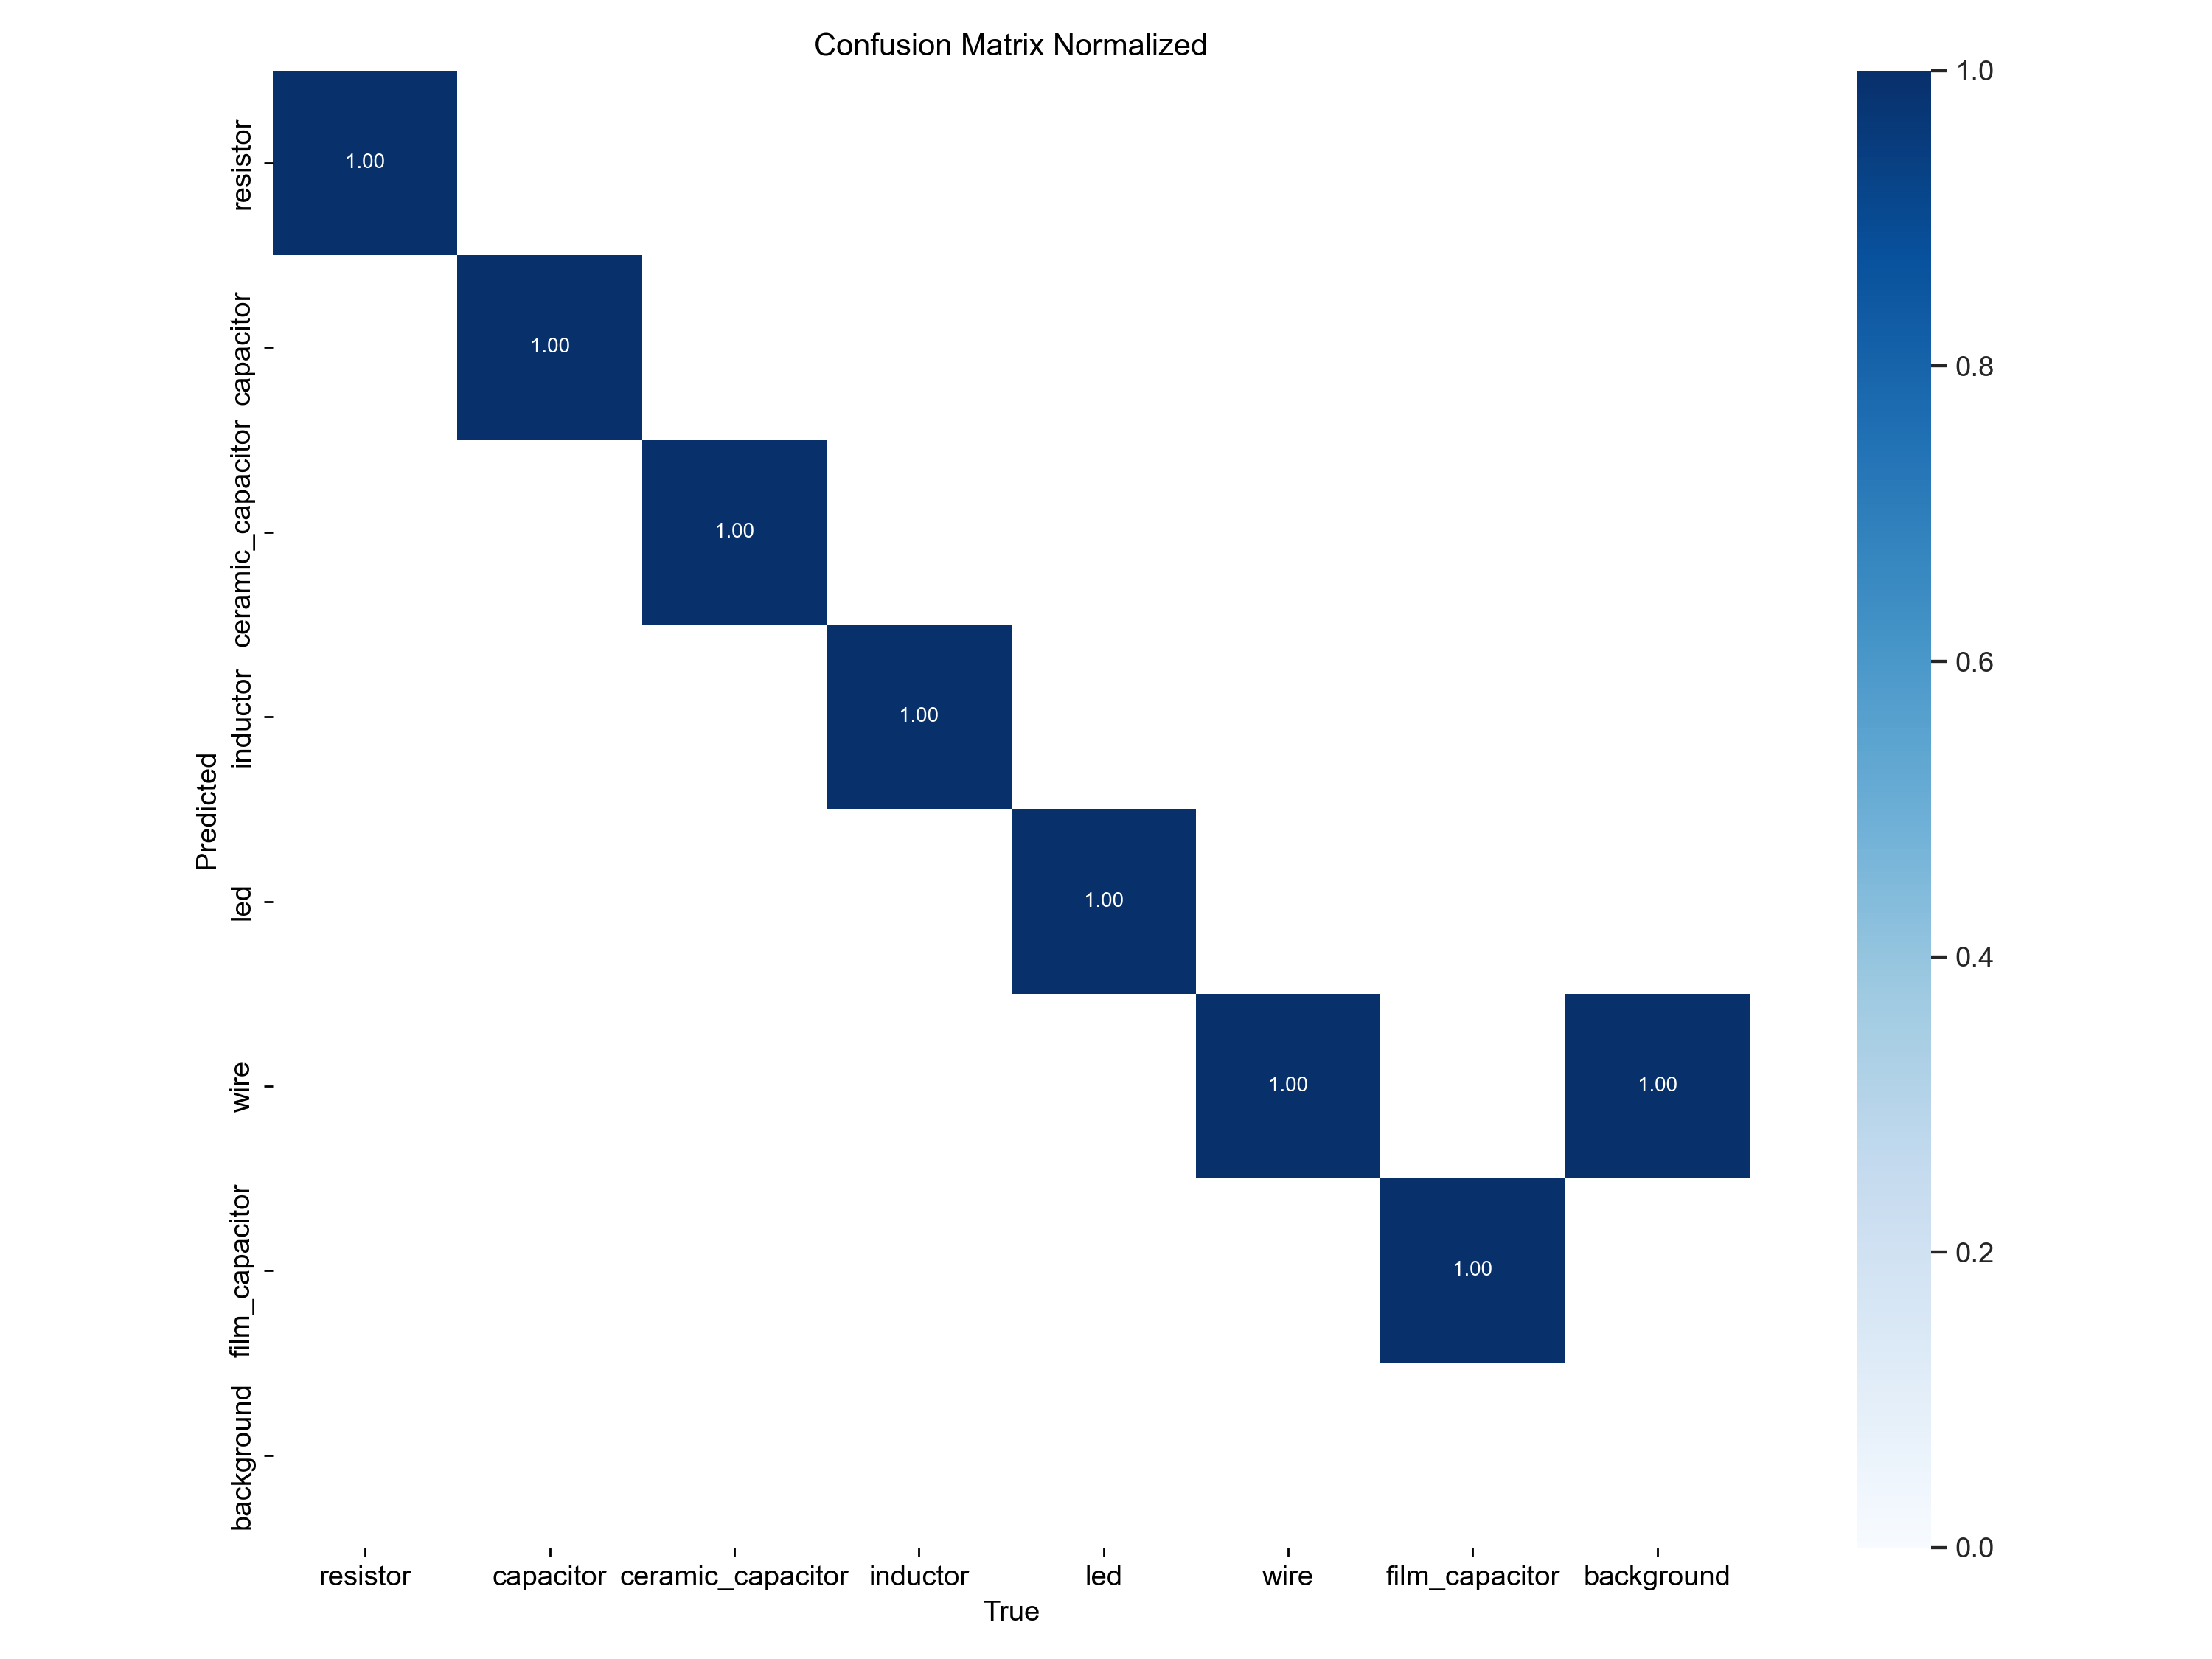
\includegraphics[width=0.8\textwidth]{imgs/graphs/confusion_matrix_test.png}
    \caption{Confusion Matrix for the test set}
    \label{fig:confusion-matrix}
  \end{figure}

During the evaluation of the model, the confusion matrix was examined to determine the model's performance on each class. The confusion matrix is shown in \autoref{fig:confusion-matrix}. Clearly, there is a strong diagonal line, which is a good sign as it shows that the model is correctly classifying most of the images, however interestingly there is a class that was unaccounted for during training; the background. 

According to the confusion matrix, the model seems to \textbf{always} place a bounding box during inference as that is what the model was trained to do; there are no images in the dataset without a component, so the model has learnt that there is always a component in the image. This is a negative side effect of the dataset, as the model has not learnt that there are images without components, and thus will always place a bounding box, which is clearly not ideal. On Ultralytics' documentation \cite{ultralytics_2023} (the creators of YOLO), they state that "0-10\% background images to help reduce FPs" and that the COCO dataset "has 1000 background images for reference", which is 1\% of the total". Luckily, this was fixed extremely easily by adding images with no labels to the dataset, and the model will learn that there are images without components.

\begin{figure}[H]
    \centering
    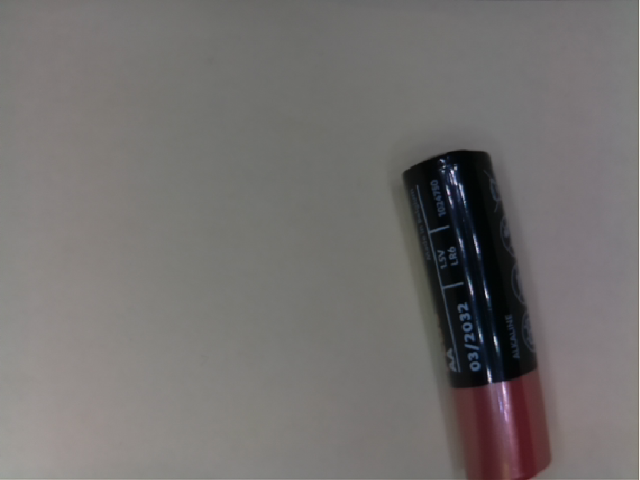
\includegraphics[width=0.8\textwidth]{imgs/cv/obb_background_1.png}
    \caption{Background image example}
    \label{fig:bg-image}
  \end{figure}
  
  As there are ~1000 images in the training set, 100 background images were added; however adding 100 images of the same static empty conveyor would not be very useful, so instead some images of the conveyor with a variety of objects were added to the dataset as shown in \autoref{fig:bg-image}, as well as other random images. The model was then retrained on this dataset, and the results are shown in. Naturally, the dataset annotation tool discussed in \label{sec:data-annotation-tool} was extended to allow for the addition of background images.
  

